
\section[{\en Cartesian Product}]{\textgreek{Η σχεσιακή πράξη του γινομένου}}
\subsection[{\en Cartesian Product}]{\textgreek{Το καρτεσιανό γινόμενο και οι εφαρμογές του}}

\begin{frame}[t, fragile, shrink]
\frametitle{Η σχεσιακή πράξη του γινομένου}
\begin{minipage}{\wE}
  \begin{block}{Ορισμός του γινομένου} \en \Large
    \[
       r \times s = \{ t \, u \, | \, t \in r \text{ and }  u \in s\}
    \]
    \el
    \large
    {\bb Καρτεσιανό γινόμενο} δύο σχέσεων $r(R)$ και $s(S)$,
    είναι μια σχέση που έχει επικεφαλίδα το σύνολο των γνωρισμάτων των σχέσεων $R$ και $S$,
    και κορμό το σύνολο όλων των συνδυασμών
    των πλειάδων που ανήκουν στην $r$ και στην $s$.
    Το καρτεσιανό γινόμενο συμβολίζεται με $r \times s$  ή {\en $r \text{ TIMES } s$}.
  \end{block}
\end{minipage}
\end{frame}


\begin{frame}[t, fragile, shrink]
\frametitle{Γνωρίσματα καρτεσιανού γινομένου}
\begin{minipage}{\wE}
  \begin{block}{Μετονομασία κοινών γνωρισμάτων}
    Το σχήμα ενός καρτεσιανού γινομένου προκύπτει μετά από μετονομασία
    των πιθανών κοινών γνωρισμάτων δύο σχέσεων. \\
    Για παράδειγμα, αν $Y$ είναι ένα κοινό γνώρισμα των σχέσεων $r(R)$ και $s(S)$,
    τότε το σχήμα της σχέσης $r \times s$ είναι:
    \par
    \large
    \[
       T = (R-S) \cup (S-R) \cup \{R.Y , S.Y \,|\, Y \in R \cap S\}
    \]
  \end{block}
\end{minipage}
\end{frame}


\begin{frame}[t, fragile, shrink]
\frametitle{Βαθμός και πληθικότητα γινομένου}
\begin{minipage}{\wE}
  \begin{block}{Βαθμός γινομένου}
    Αν η σχέση $r$ είναι $n_R$ βαθμού
    και η σχέση $s$ είναι $n_S$ βαθμού τότε το αποτέλεσμα του γινομένου έχει βαθμό:
    \[
       n_{r \times s}  = n_R + n_S
    \]
  \end{block}
  \begin{block}{Πληθικότητα γινομένου}
    Αν η σχέση $r$ είναι $m_r$ βαθμού
    και η σχέση $s$ είναι $m_s$ βαθμού τότε το αποτέλεσμα του γινομένου έχει βαθμό:
    \[
       m_{r \times s}  =m_r \cdot m_s
    \]
  \end{block}
\end{minipage}
\end{frame}



\begin{frame}[t, fragile, shrink]
\frametitle{Παράδειγμα σχεσιακού γινομένου}
\begin{minipage}{\wE}
  %\begin{block}{}
\en
\begin{tabular}{ c c c }
  $r$ & $s$ & $r \times s$ \\
  \begin{tabular}{ c c } \toprule
    {\bf A} & {\bf B}  \\            \midrule
    1 & b  \\
    5 & a  \\
    3 & c  \\            \bottomrule
      &    \\
      &    \\
      &    \\
  \end{tabular}
&
  \begin{tabular}{ c c c }  \toprule
    {\bf D} & {\bf E} & {\bf F} \\ \midrule
    b & 4 & 30 \\
    a & 2 & 10 \\ \bottomrule
      &    \\
      &    \\
      &    \\
      &    \\
  \end{tabular}
&
  \begin{tabular}{ c c c c c }  \toprule
    {\bf A} & {\bf B} & {\bf D} & {\bf E} & {\bf F}  \\ \midrule
    1 & b & b & 4 & 30 \\
    1 & b & a & 2 & 10 \\
    5 & a & b & 4 & 30 \\
    5 & a & a & 2 & 10 \\
    3 & c & b & 4 & 30 \\
    3 & c & a & 2 & 10 \\    \bottomrule
  \end{tabular}
\\
\end{tabular}
\el
  %\end{block}
\end{minipage}
\end{frame}



\begin{frame}[t, fragile, shrink]
\frametitle{Γινόμενο και μετονομασία γνωρισμάτων}
\begin{minipage}{\wE}
\en
\begin{tabular}{ c c c }
  $r$ & $s$ & $r \times s$ \\
  \begin{tabular}{ c c } \toprule
    {\bf A} & {\bf B}  \\            \midrule
    1 & b  \\
    5 & a  \\
    3 & c  \\            \bottomrule
      &    \\
      &    \\
      &    \\
  \end{tabular}
&
  \begin{tabular}{ c c c }  \toprule
    {\bf A} & {\bf B} & {\bf F} \\ \midrule
    b & 4 & 30 \\
    a & 2 & 10 \\ \bottomrule
      &    \\
      &    \\
      &    \\
      &    \\
  \end{tabular}
&
  \begin{tabular}{ c c c c c }  \toprule
    {\bf R.A} & {\bf R.B} & {\bf S.A} & {\bf S.B} & {\bf F}  \\ \midrule
    1 & b & b & 4 & 30 \\
    1 & b & a & 2 & 10 \\
    5 & a & b & 4 & 30 \\
    5 & a & a & 2 & 10 \\
    3 & c & b & 4 & 30 \\
    3 & c & a & 2 & 10 \\    \bottomrule
  \end{tabular}
\\
\end{tabular}
\el
\end{minipage}
\end{frame}


\begin{comment}
\begin{frame}
\frametitle{Ιδιότητες του γινομένου}
\begin{block}{Αντιμεταθετική ιδιότητα}
\[
r \times s = s \times r
\]
Δηλαδή δεν έχει σημασία η σειρά των τελεσταίων, με οποιαδήποτε σειρά και να γίνει η πράξη
της τομής το αποτέλεσμα είναι το ίδιο.
\end{block}
\begin{block}{Προσεταιριστική ιδιότητα}
\[
r \times (s \times t) = (r \times s) \times t
\]
\end{block}
\end{frame}

\begin{frame}
\frametitle{Παράδειγμα γινομένου με σύνολα}
Αν
\[ A=\{a,b,c\} \]
και \[ B=\{1,2\}\]
τότε
\[
Α \times B = \{(a,1), (a,2), (b,1), (b,2), (c,1), (c,2) \}
\]
Δηλαδή το γινόμενο δύο συνόλων $A$ και $B$ αποτελείται από όλους
τους συνδυασμούς των μελών των $A$ και $B$.
\end{frame}
\end{comment}


\begin{frame}[t, fragile, shrink]
\frametitle{Δενδροειδής απεικόνιση καρτεσιανού γινομένου}
\begin{minipage}{\wE}
  \begin{columns}[T]
    \begin{column}{0.5\textwidth}
      \en
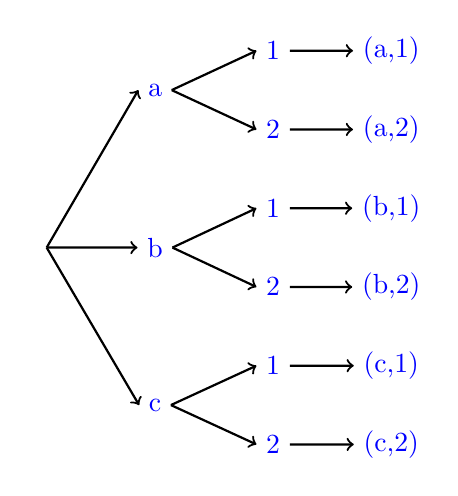
\begin{tikzpicture}
  [parent anchor=east,child anchor=west, grow=east, 
  every node/.style={circle,draw},  
  level 1/.style={sibling distance=20mm},
  level 2/.style={sibling distance=10mm},
  level 3/.style={sibling distance=10mm},
 ]
  \tikzstyle{every node}=[text=blue]
  \tikzstyle{edge from parent}=[draw, ->, solid, thick, black]
\node { }
  child {node {c} 
    child {node {2} child {node {(c,2)}} }
    child {node {1} child {node {(c,1)}} }
  }
  child {node {b} 
    child {node {2} child {node {(b,2)}} }
    child {node {1} child {node {(b,1)}} }
  }
  child {node {a}
    child {node {2} child {node {(a,2)}} }
    child {node {1} child {node {(a,1)}} }
  };
\end{tikzpicture}
\el

    \end{column}
    \begin{column}{0.5\textwidth}
     \begin{align*}
       A &=& \{a,b,c\} \\
       B &=& \{1,2\}  \\
       A \times B &=& \{ (a,1), (a,2) \\
                  &&     (b,1), (b,2), \\
                  &&     (c,1), (c,2) \}
     \end{align*}
    \end{column}
  \end{columns}
\end{minipage}
\end{frame}


\begin{frame}[t, fragile, shrink]
\frametitle{Απεικόνιση καρτεσιανού γινομένου σε σύνολα}
\begin{minipage}{\wE}
  \begin{columns}[T]
    \begin{column}{0.5\textwidth}
      \begin{tikzpicture}
  \tikzstyle{every state} = [fill, draw=black, blue50, text=black]
  \tikzstyle{every state} = [inner sep=0.5pt, minimum size=0pt, scale=0.9]
   
  \def\A{0.0};
  \def\B{3.0};

  \draw (\A, 0) ellipse (22pt and 36pt); % A
  \draw (\B, 0) ellipse (22pt and 36pt); % B

  % A nodes
  \node[state] (a1) at (\A,  20pt) {$a$};
  \node[state] (a2) at (\A,   0pt) {$b$};
  \node[state] (a3) at (\A, -20pt) {$c$};

  % B nodes
  \node[state] (b1) at (\B,  16pt) {$1$};
  \node[state] (b2) at (\B, -16pt) {$2$};

  % connection lines
  \path[-] (a1) edge  (b1);
  \path[-] (a2) edge  (b1);
  \path[-] (a3) edge  (b1);
  \path[-] (a1) edge  (b2);
  \path[-] (a2) edge  (b2);
  \path[-] (a3) edge  (b2);
  

  % annotate names
  \draw (\A, 45pt) node {\large$\mathbf{A}$};
  \draw (\B, 45pt) node {\large$\mathbf{B}$};

\end{tikzpicture}

    \end{column}
    \begin{column}{0.5\textwidth}
     \begin{align*}
       A &=& \{a,b,c\} \\
       B &=& \{1,2\}  \\
       A \times B &=& \{ (a,1), (a,2) \\
                  &&     (b,1), (b,2), \\
                  &&     (c,1), (c,2) \}
     \end{align*}
    \end{column}
  \end{columns}
\end{minipage}
\end{frame}



\begin{frame}[t, fragile, shrink]
\frametitle{Προσοχή στο καρτεσιανό γινόμενο}
\begin{minipage}{\wE}
  \begin{exampleblock}{Φοιτητές και Μαθήματα}
    Αν $M$ είναι το σύνολο των μαθημάτων 
    και $\Phi$ είναι το σύνολο των φοιτητών 
    τότε
    \vspace*{-0.5cm} \[ M \times \Phi \]    %\vspace*{-0.5cm}
    είναι ο συνδυασμός όλων των μαθημάτων με όλους τους φοιτητές
    (όλοι εξετάζονται σε όλα).
  \end{exampleblock}
  \begin{exampleblock}{Ηθοποιοί και ταινίες}
    Αν $H$ είναι το σύνολο των ηθοποιών
    και $T$ είναι το σύνολο των ταινιών
    τότε \vspace*{-0.5cm}    \[ H \times T \]    %\vspace*{-0.5cm}
    είναι ο συνδυασμός όλων των ηθοποιών με όλες τις ταινίες
    (όλοι παίζουν σε όλες).
  \end{exampleblock}

\end{minipage}
\end{frame}
